\documentclass[11pt,letter]{article}
\usepackage[top=1.00in, bottom=1.0in, left=1.1in, right=1.1in]{geometry}
\renewcommand{\baselinestretch}{1.1}
\usepackage{graphicx}
\usepackage{natbib}
\usepackage{gensymb}
\usepackage{amsmath}

\def\labelitemi{--}
\parindent=0pt

\begin{document}
\bibliographystyle{/Users/Lizzie/Documents/EndnoteRelated/Bibtex/styles/besjournals}
\renewcommand{\refname}{\CHead{}}
\begin{flushright}
Version dated: \today
\end{flushright}
\bigskip
\noindent RH: Interactive cues and spring phenology
% put in your own RH (running head)

\bigskip
\medskip
\begin{center}

% Insert your title:
\noindent{\Large {\bf Concept paper on understanding interactive cues and climate change (with growth chamber studies)}}\\
\vspace{2ex}
{\Large (1) How interactive cues will shape climate change responses \\
\vspace{2ex}
(2) Limiting cues: How spring warming, winter chilling and daylength will shape climate change responses\\
\vspace{2ex}
(3) Spring warming, winter warming or daylength: What cue will be most limiting in future tree phenology?} % What cue will be most limiting with climate change? Forcing x photoperiod x chilling
% Isabelle likes 3 best.
\bigskip

\noindent {\normalsize \sc
The lab$^{1,2}$}\\ % Ailene, Cat, Dan, Lizzie, Nacho
\noindent {\small \it
$^1$ Arnold Arboretum of Harvard University, 1300 Centre Street, Boston, Massachusetts, 02131, USA\\
$^2$ Organismic \& Evolutionary Biology, Harvard University, 26 Oxford Street, Cambridge, Massachusetts, 02138, USA\\
$^3$ Forest \& Conservation Sciences, Faculty of Forestry, University of British Columbia, 2424 Main Mall, Vancouver, BC V6T 1Z4}\\

\end{center}
\medskip
\noindent{\bf Corresponding author:} Lizzie, see $^{1,2}$ above ; E-mail:.\\

\newpage
%\linenumbers

\begin{abstract}
Climate change has shifted plant phenology globally, with average shifts of 4-6 days$\degree$ C and some species shifting several weeks. Globally, such shifts have been some of the most reported and most predictable biological impacts of climate change. This predictability comes from decades of research, which have outlined the major cues that drive most studied plant phenology: temperatures (including spring warming and winter chilling) and daylength. Further simplifying predictions, spring temperatures are often the dominant cue in nature, making linear models of heat sums often excellent at predicting interannual variation in phenology. Yet as climate change has marched on, new research has uncovered possible failures to predict the current observed changes, with many shifts appearing more muted over certain time periods or in certain locations. Here we argue that some of these inaccurate predictions are due to simple models that neglect to consider other major cues---especially winter chilling and daylength, which moderate and shape plant phenological responses to spring warming. We highlight how over 60 years of research in controlled environments can improve predictions for when, where and how the interactive effects of other cues will impact simple linear predictions. Finally, we discuss how a new generation of controlled environment experiments could rapidly improve our predictive capacity for woody plant phenology in coming decades.  
\end{abstract}

\noindent \emph{Main message (and, really, it's important):} If you want to project climate change impacts, you need to focus on relevant changes in all three cues. The relevant changes part is about comparing cues, the all three cues is about interactive cues.

\noindent \emph{Keywords:} phenology, climate change, spring warming, forcing, chilling, daylength, photoperiod, non-linear responses, leafout, budburst\\

\newpage
\section{Main text}
Shifts in spring plant phenology are one of the most reported and most predictable changes with climate change. Decades of research have documented advancing budburst, leafout and flowering across systems \citep{delpierre2009, yu2010,Ellwood2012,jochner2013,hereford2017}, especially in temperate systems where long-term records have made an especially strong case for how humans have altered the timing of spring \citep{Schwartz:1997nn,Menzel2003a,Menzel:2006sq}. Recently, however, these advances have appeared to slow \citep{fu2015} or even reverse in some places \citep{yu2010}, and failing to fit simple predictions of and advancing spring with continued warming \citep{Ellwood2012}. The main hypothesis for this failure is that a plant cue to spring warming---which most observational studies focus on---is no longer the only cue that matters to predicting responses to continued warming \citep{chuine2016}.\\ % check Cat's work at mini-retreat in June for more citations!

Despite the focus of much spring phenology researach on spring warming cues the underlying physiology of phenology is much more complicated. For many species three major cues drive spring phenology: forcing (warm temperatues, generally occurring in the late winter and early spring), chilling (cool temperatures, generally occurring in the fall and winter), photoperiod (daylength). Forcing and chilling cues are generally understood to be accummulation processes, where plants must integrate chilling and forcing experienced over time to meet a sum threshold value at which they can budburst, leafout or flower. In contrast, photoperiod is generally not an integral cue, but one evaluated daily. These cues together may create critical non-linear responses that many current methods cannot predict. [TRANSITION?]\\

Measuring these three major cues and understanding how they will interactively determine current and especially future phenology is hard for several major reasons. First, these cues vary across species, and possibly within species across the range  \citep{vitasse2009,harrington2015}. Second, the cues appear designed to interact: one cues may compensate for another cue. In practice this means studies that are not desigend to tease apart these cues experimentally (e.g., observational studies) may find statistical evidence for only one cue, because it masks one other cues. For example, a plant that have not received enough chilling would generally require more forcing and thus leafout later, which could look indistinguishable from a photoperiod requirement that has not been met. To some extent the interactions of these cues have meant that---for many locations in most years---researchers have not been challenged to measure cues beyond forcing to understand advances and make accurate near-term predictions. In many locations if chilling cues are met and forcing produces budburst at an acceptably long photoperiod---then the main cue needed for predictions is simply forcing, and simple linear models of spring warming versus spring phenology may suffice. But, increasing evidence, in some systems in some years, suggests these chilling and photoperiod may play an important role in spring phenology today, with that importance growing in the future. If rising evidence suggests these cues are critical to understand current responses and predict future non-linearities, then how do we integrate them more into phenological research? \\% Thus, the cues in obervational data---even long-term records---can be very hard to measure. 

The first step towards improved phenological predictions is robust measurements of chilling, forcing and photoperiod cues. Recently, much effort has focused on estimating these cues from long-term observational data. Yet obsverational data may often fail to robustly estimate any of the three major cues due to two types of statistical issues. First, in most observational data these cues are effectively correlated: forcing increases alongside longer days, and the response to a high chilling cue is the same predicted for a strong photoperiod cue (i.e., later spring phenology). Secondly, most observational studies focus on linear models of each cue and often without interactions between cues. This is perhaps unsurprising as the non-linearities in most plant phenological responses to most cues are expected to be linear except at extremes (and natural conditions often see only a small slice of the range of values of each cue that are possible), and given that interactions between cues are difficult to estimate---moreso when those cues are highly correlated in nature. The one method designed to robustly measure these cues is controlled environment (e.g., growth chamber) studies \citep{nagano2012,satake2013}.\\

Growth chamber studies of plan phenology have conducted for over 70 years and are specifically designed to understand non-linearities both in individual cues and produced by interactions between cues. In contrast to observational studies, controlled environment studies can manipulate all three cues, and extend to other cues that may important in some species or biomes (e.g., humidity, drought conditions, light spectra), and can tease out interactions between cues by experimentally decoupling them. Despite the prevalence of growth chamber studies for spring phenological cues, they have rarely been reviewed. Perhaps more suprisingly, they have been often poorly integrated into the current phenological literature on climate change. This includes in debates where they are critical---such as about the importance of photoperiod (CITES, incl Richardson).\\

Here we aim to help integrate the long-term literature on growth chamber studies into current phenological research on climate change more fully. We begin with a brief review how three major phenological cues for woody plant phenology will shift in coming decades with anthropogenic climate change. We then review 70 years of study on the three major phenological cues from growth chamber studies, with a particular aim to understand how much of the cue-space has been studied and how experimental treatments compare to shifts in cues caused by climate change. Based on this, we discuss how growth chamber studies can be best designed to understand these interactive cues and build more robust predictions.\\

Given our aim to improve understanding of current trends and forecasts we focus on early vegetative phases (budburst and leafout) of wild species, which are critical to plant growth and thus to models of carbon uptake and storage. We touch on other areas of research, which have been important to our understanding of the cues underlying phenology. In particular, research has been especially strong in model systems (e.g., \emph{Arabidopsis, Populus}) and crops \citep{cesaraccio2004}---with the exact phenophase of interest varying (potentially by a species' life history: more focus on germination and flowering in \emph{Arabidopsis}, and more on leafout and budset in \emph{Populus}).  Given our focus on budburst and leafout, our review concentrates on woody species phenology, where most research has been conducted. Most of our conclusions and suggested approaches, however, could equally apply to non-woody species and/or other phenophases with underlying similar interactive cues.\\ 
% \citep{primack2015}
\subsection{How will chilling, forcing and photoperiod shift with climate change?}
Before examining how chilling, forcing and photoperiod will shift with climate change, it helps to review why species have multiple environmental cues for spring phenology---to cope with the environmental variation each species experiences across its range and across years. In the spring, selection for species to track the start of resources each year (to gain access to them before other individuals have depleted them) means that species need cues that work across the interannual variation in climate across of their ranges. This variation can come from either plasticity and/or local adaptation. Spring phenology can be fairly plastic (CITE). Especially compared to other phenophases, such as budset phenology, budburst and leafout often do not show high local adaptation across a range (CITESAItken). This means that species ideally need a set of cues that work across their range \citep{liepe2016}, though there may be variation in the importance of each cue across a range (e.g., chilling can be higher in coastal versus continental, check also \citet{legave2013}), and genetic work suggests the same genes can be triggered by very different enviromental cues (e.g., vernalization cues in \emph{Arabidopsis thaliana} CITE). Cues for species with high climatic variation across their ranges will thus need cues adapted to high climatic variation (spatially and temporally).\\

Temperate species that employ three cues---forcing, chilling, photoperiod---provide many diverse paths to budburst each season, especially through interactions between these cues and/or non-linearties in certain cues. Indeed, one of the most critical changes that can happen is when pre-climate change conditions generally caused budburst to occur at the extremes of some cues (e.g., high chilling and/or long photoperiods, where responses may be effectively muted, see FIGURE?) and climate change has now pushed budburst into periods where these cues are at the more linear part.\\ % Some major problems in terminology here -- cue versus response!

All three major cues are expected to shift with climate change (See Fig. \ref{fig:pep}), though the shifts will vary substantially across space and time. Most notably to date, warming increases the forcing plants experience each day (CITES), with more rapid shifts---and thus also greater shifts---at higher elevations and in the arctic (CITES). [Give range of warming depending on different scenarios!]. Daily minima (generally night-time temperature) will; generally warm more than maxima temperatures, though this effect varies spatially (CITES). Warming across seasons is also variable (ADD more here). \\
% Note \citet{piao2015}- found that daytime forcing temperatures (Tmax) are more important for leaf out than nighttime temperatures (Tmin). Any other citations about this? I imagine there must be more. 
Warming also translates into important shifts in chilling, though a dearth of understanding on chilling makes predicted shifts in chilling complicated. Research to date suggests chilling only accumulates in a certain range of temperatures with low (e.g., $<$0$\degree$C) temperatures generally not contributing to chilling accumulations and higher temperatures (e.g., $>$12$\degree$C) potentially decreasing previously accumulated chilling. Thus, major shifts in accumulated chilling would be predicted where temperature regimes that were previously too low to accumulate chilling in many months of the winter warm such that chilling now accumulates in those months (CITES). Areas with this shift would then expect much earlier budburst with warming, potentially far earlier than last frost dates (CITES). Unfortunately, these predictions are based on models developed almost solely for agricultural crops (but see HARRINGTON CITES etc.), especially stone fruits, and have rarely been robustly adapted to forest trees. While the development of classic models of chilling for peaches and related fruit trees benefited from data on these species being planted far outside their range into regions with extremely low or potentially no chilling, equivalent data on forest trees is almost never available. Thus chilling models to date generally use limited observational and experimental data from forest trees to try to reparametrize the basic stone fruit models (CITES).\\

Improved chilling models for forest trees (and horticultural trees) may come from an improved understanding of dormancy at the physiological level. Chilling is defined as what leads to break of endodormancy (DEFINE/check this definition), after which plants enter ecodormancy when accumulated forcing then leads to budburst. Measuring endodormancy and its transition into ecodormancy is notoriously difficulty, however, and work to date has relied generally on cellular staining methods tested on a very limited subset of species (CITES). These methods themselves rely on a still-developing understanding of what causes dormancy at the cellular level (CITES). In practice, most phenology studies use the terms `chilling' and `forcing' to mean `cool temperatures' (often either in the fall and winter or applied first in experimental conditions) and `warm temperatures' (often either in the spring or applied after sufficent chilling) and generally hope they correspond to endo- and eco-dormancy. Some studies use the sequential transfer of cuttings to warm conditions to estimate the transition from endo- to eco-dormancy, with rapid and full (e.g., $>$90\% of buds on a cutting) budburst generally meaning a plant is ecodormant, but given that this is labor- and space-intensive most studies considering chilling do not do this. We expect that without a much improved physiological understanding of endo-dormancy release robust models of chilling---and thus accurate predictions of how chilling will shift with climate change---will be difficult to develop. \\ % And there is so much we don't know about how chilling works and interacts with forcing (sequential model, parallel models etc.)

Research has discussed shifts in photoperiod with climate change far less often compared to predicted changes in forcing and chilling (but see CITES). While an environment's photoperiod does not shift with climate change, the relevant photoperiod a plant experiences at critical physiological points may change dramatically with warming. In particular, increases in chilling and/or forcing, which could alone produce much earlier budburst, may be offset by short photoperiods (CITES) that delay budburst. Similarly, long photoperiods can lead to budburst sooner than predicted by solely low chilling or forcing conditions (CITES). Thus, changes in chilling and/or forcing correspond to changes in the relevant photoperiod with climate change. \\
% although daylengths themselves won't change with climate change, the photoperiods experienced by organisms are likely shift as ranges shift and phenology shift (cite our other paper?)

These cues may create non-linear responses with warming in three major ways. First, as discussed above, each cue may be non-linear alone. For example, cues may be linear in the mid-range of values, while extremely high or low values of some cues (e.g., photoperiod) may produce alternative response. For example, at very low photoperiod (short days) plants often will not grow, similarly maximum growth may occur at photoperiods of 18 hours, meaning photoperiods longer than 18 hours will have no additional effect on budburst timing.  % see Gauzere
Secondly, interactions between cues can produce non-linearities. For example, if forcing and photoperiod both determine budburst timing and have a subadditive interaction (i.e., both cues together produce a more muted response than the addition of each cue's effect alone) then the two cues together will produce a non-linear response. The interaction of interactive cues with common environmental correlations may cause additional non-linear complexities (e.g., warm springs may cause mean plants meeting their forcing cues at shorter photoperiods). \\

Given our current understanding of phenological cues, we should expect the most dramatic changes in phenology in systems with non-linear responses where climate change pushes the system across a critical threshold or inflection points. For example, if some species have a critical photoperiod for budburst and warming means forcing cues are met before the critical threshold, then we would expect incomplete or highly delayed budburst (CITES). Similarly the complexity of chilling could produce myriad non-linearities. If, as currently hypothesized, chilling follows an optimum curve (i.e., chilling does not accumulate at very low or high temperatures but in between it accumulates at a maximum rate at some temperature optimum), then endodormancy break would shift earlier in systems where warming pushes winter temperatures into a chilling-accumulation temperature or closer to the optimum temperature, and delay where warming pushes winter temperatures beyond the optimum (with more complex predictions if high temperatures decrease accumulated chilling). Interactive cues could also produce non-linear responses, but predicting these requires a refined understanding of the interaction and whether there are critical inflection points that may crossed with continued warming. These complexities highlight how difficult predictions may be without careful efforts to tease out how each cue works alone and interactively. 

\subsection{Predicting non-linear responses with controlled environment experiments} % or just forecasting future responses?

Controlled environment (generally growth chamber students) can help predict non-linear responses by allowing researchers to examine the effects of one cue with the others held constant, and examine interactive effects (given the appropriate study design). Such experiments may be especially useful for forecasting if they are designed in a range relevant to current versus future conditions. Indeed, one of the major advantages of experiments is that they allow treatments outside of the historical range---an option long-term observational data can never provide. We reviewed controlled environment studies over the last seven decades (1947-2014) to understand the range of treatments already available, and how they compare to current and future conditions. We note that these studies were rarely conducted for climate change research, and most often done for fundmental science or other areas of applied science (e.g., horticulture or forestry). Nevertheless, they are some of the best available data for how plants respond to the environment and thus a critical resource for climate change research today.\\

% Need to update below once Cat updates table ... 
Controlled environment studies have been conducted across 227 species across the globe, with the majority of papers report research occurring in Europe (54 of 91 papers), followed by North America (23, Fig. \ref{fig:datamap}). Most studies manipulate one cue (Fig. \ref{fig:ts}), though studies of two or three cues have occurred in almost every decade. Forcing and photoperiod were the most commonly studied cues (56\% manipulated forcing; 55\% manipulated photperiod), with chilling being studied in only a third of all studies (33\% manipulated chilling). The actual cues studied varied across latitude with a general trend toward examining more extreme values at higher latitudes. Thus, forcing and chilling treatments ($\degree$ C) declines 0.1$\degree$C per $\degree$ latitude (for forcing, min is -0.12, for max it's -0.08, see Fig \ref{fig:lat}; for chilling it's -0.1 for min and -0.07 for max); and the maximum studied photoperiod increases with latitude (0.08 hr per degree $\degree$ latitude). These shifts across space make sense---higher latitudes experience colder temperatures and longer photoperiods---but introduce a bias in results as any comparisons of studies from lower and higher latitudes are also comparing a different range of cues generally. \\
% Need to add: 
% (1) Table of all analyses here
% (2) Say something about material (seeds/saplings/cuttings)? Can we tie to relevance of predicting future forest communities or such?


Single cue studies were the most common, but prevent understanding interactions among cues or comparisons of which cues dominate phenological responses; studies of multiple cues can overcome these challenges. [NEED TO CHECK] Of the studies manipulating at least one cue, half additionally manipulated another cue. Study designs most often allowed examining whether cues were interactive (that is, whether the effect of one cue depends on the level of the other cue), with the most studies testing for interactions between photoperiod and forcing (14 studies), followed by studies that examined the effects of photoperiod (12) and forcing (11) across the fall-winter. Such studies follow the design generally attributed to Weinberger (CITE) where tissue (e.g., cuttings) are taken progressively across the fall and/or winter seasons then exposed to controlled environment conditions. These studies often equate tissue removed later from the field as having received more chilling and thus often treat `time of cutting' as interchangeable with `chilling' though forcing and photoperiod conditions also change along a temporal gradient. Studies examing photoperiod or forcing crossed with experimental chilling treatments (either through changes in temperature or days of chilling) were slightly less common (8 studies each for photoperiod and forcing). Studies examining three cues directly were very rare: we identified only two studies examining all three cues at once, and both were on \emph{Picea abies} (CITE). A slightly larger set of studies (five) examined three cues indirectly---manipulating photoperiod and forcing in controlled environments but equating chilling with sequential removal of tissue from the field---for 11 species (CITES). \\
% I think we need to add what the interactive studies found -- did they all find interactions? 
% "okie11_exp2"  -- Peach, doesn't really cross forcing (mainly chill x photo)   "worrall67_exp 3" (this paper coolly opens with "As has been repealedly empha.sized in the literature, discussion.s of dor- mancy in woody plants are often misleading becatise of the lack of a standard nomenclature.") and "sogaard08_exp2" .... both on Picea abies
% "basler14_exp1" (Acer pseudoplatanus. Fagus sylvatica, Quercus petraea, Picea abies)  "heide93_exp1"    "heide93_exp2" (heide93 was Alnus incana, Alnus glutinosa, Populus tremula, Prunus padus, Betula pubescens, Betula pendula)  "partanen98_exp1" (Picea abies) "schnabel87_exp1" (Vitis vinifera) -- all checked

The paucity of studies examining multiple cues limits our fundamental understanding of each cue, as well as how---when combined---they will play out to determine future leafout with continued warming. Because the cues are all known to be interactive, estimates of any one cue are influenced by the level of each other cue. Knowing the level of each other cue is difficult both because they are often not reported, and also because they are somewhat impossible to know given our current understanding of endodormancy (when we understand chilling is applied) and ecodormancy (when we understand forcing is applied). Authors may use the terms `chilling' and `forcing' for their treatments, but they rarely have physiological evidence that these are the actual treatments being applied. Studies using sequential removal from the field to estimate chilling are at perhaps the greatest disadvantage to estimate the cues applied: chilling must rely field estimates of from models that are currently only hypotheses of actual chilling, and forcing and photoperiod treatments are most probably a mix conditions in the field and conditions applied in controlled environments. Further any study conducted over much of the fall and winter is most likely estimating the effect of their `forcing' and photoperiod treatments on first endodormant plants, and then ecodormant plants---with when the switch happened generally unknown. Some studies do attempt to assess dormancy state ... [we need to add more here!]. [... end on needing more studies of interactive cues or just more studies reporting dormancy state and best guess at other cues?]\\

% START HERE! When possible I also need to ..
% Finish the countinxns code and make the heatmaps.
% Review Weinberger and chilling studies in general
% Decide what to call cues/levels of cues etc. Gauzere says cue for presence of a response (e.g., to photoperiod) ... they also use `compensatory effects of chilling on forcing requirements' ... as a way to subadditive I believe. They seem to describe the underlying curves as responses (e.g., `chilling and forcing responses') ... hmm, but they also say stuff like: "the effective response to day length simulated by the models can highly differ according to the adjusted reaction norms" so maybe response curve and reaction norm are interchangeable?
The utility of controlled environment studies to forecasting also depends on how relevant treatments are to current and future conditions. Estimating such relevance is difficult as it depends on a species' range and projections considered, however, our best attempt at this for two widely studied species \emph{Fagus sylvatica} and \emph{Betula pendula} suggest experiments have generally bracketed the range of projected temperatures ...

% Need to include something about how similar to nature these treatments are!





\begin{enumerate}
\item Growth chamber studies should help predict both these non-linearities. This is especially useful for forecasting if they are designed in a range relevant to current and future conditions: Compare treatments from controlled environment studies to predicted shifts in cues with climate change: {\bf Part I: Review of the three major phenological cues from growth chamber studies over the last 67 years} % 2014-1947
\item X\% of studies manipulated which interacting cues? (i.e., how many studies manipulate 1 cues, 2 cues, 3 cues ... of those manipulating 1 cue, what is the breakdown by cue etc.) ... 43\% manipulated forcing and photo, only 10\% manipulated chilling and forcing or photo (9\% for chill x photo; 10\% for chill x force), see Fig. \ref{fig:heatmaps}
\item Compare treatments from controlled environment studies to predicted shifts in cues with climate change: {\bf Part II: What cues will be most limiting with climate change? How do controlled environment studies compare?}
\begin{enumerate}
\item Consider both the range of a species and the climate change projections ...
\begin{enumerate}
\item Take each PEP725 datapoint within our selected species' range and calculate:
\begin{enumerate}
\item Do we really have negative forcing in OSPREE? (See Fig. \ref{fig:pep})
\item Experiments have done a good job of testing chilling compared to climate change projections, covers full range and overshoots a bit ... (See Fig. \ref{fig:pep}) \footnote{We used daily min/max, as they're most directly comparable to OSPREE.}
\end{enumerate}
\end{enumerate}
\end{enumerate}
\end{enumerate}

\subsection{Path forward}

\begin{enumerate}
\item Paths forward (showcase how growth chamber studies can be best designed to better understand these interactive cues in regards to climate change forecasting) 
\begin{enumerate}
\item If you want work to be most relevant to climate change, then consider the following when designing experiments:
\begin{enumerate}
% Now that climate change is here, experiments that want to claim climate change relevance must address what the cue impacts of climate change will really be
\item The cues with the current vs. future range of a species (as we did above) to inform experimental range % Isabelle: species are expected to follow their climatic niche, so basically they will remain in the same climatic conditions. This point becomes important for trailing edge populations that might be able to remain several years in non optimal conditions.
\item If you don't work within the range or projected cue range limits of a species, then consider working on informative extremes to help identify where single-cue non-linearities exist... but some extremes (e.g., chilling) are difficult to reproduce in controlled environments (and this is something we technologically need to improve)
\end{enumerate}
\item Manipulating more than one cue may be most useful, esp. if we want to understand interactive cues and advance comparisons with long-term data 
\item Major need to better understand deviations in long-term data are: better non-linear models for more species. How best to do this?
% (Cat:) Personally I think this is so important! Citizen Science programs for phenology are expanding. I know the NPN is growing and major NGOs are trying to incorporate more phenology data. Phenology is also growing in the media, thus, I think it’s essential we include this. I like that it is brief but , for me, the major take away of the paper is that we are aiming to encourage phonologists, in general, to make improvements. 
\begin{enumerate}
\item Studies using only long-term observational data have already improved in being clear about correlations in predictor variables (e.g., chilling, forcing and daylength often covary). This means we generally cannot robustly identify other cues through statistical modeling and need alternative approaches... % AKE: Also add: can we use any long-term observational data to look at interactive cues at all? for example, elevational gradient studies or gradients/locations with small scale  but strong microclimate variations (photoperiod should be consistent- more or less- though forcing and chilling might be quite different, for example). % EMW: I thought about this and looked at Yann's elevational work -- but he saw strong local adapation so I am not sure what you can do with long-term data without knowing the underlying genetic changes/differences as well. 
\item A better option than just long-term data are more efforts to integrate long-term data with growth chamber studies \citep{Caffarra:2011qf,nagano2012,satake2013,ford2016,chuinearees} % The ford et al paper on doug-fir that i listed above (see above) is an example of integrating growth chambers with long-term provenance trials.
\begin{enumerate}
\item Studies that test the extremes are needed to parameterize models (ideally you need to know where the zeros are) \citep{chuinearees} % Nacho says: thermal tolerances may impose an ultimate filter to discard survival of a species under too cold-warm conditions, but an earlier, perhaps more informative filter is provided by phenology.
\item Traditional methods to hold-out data and test how well the model performs
\item Use growth chamber studies to test model predictions, especially in future climate scenarios where non-linearities are predicted, and vice versa \citep[see][]{nagano2012}
\item Improving models means more back-and-forth worth between developing models based on both long-term data and experiments, then testing predictions with new experiments and as newer observational data are generated (i.e., more years and also data from new locations) ... \citep{nagano2012,satake2013}
\end{enumerate}
\end{enumerate}
\item Building species-rich predictions ... 
\begin{enumerate}
\item Given how complicated this all sounds, how do we build up to multi-species predictions?
\item Need more efforts to combine data
\item Introduce Bayesian hierarchical modeling within this framework
\item And need more efforts to publish studies in a way that makes synthesis possible ...
\item Studies not interested in climate change forecasting can still contribute---with little effort---to progress in this area by: Reporting all cues (even the ones you don't measure) so they can be used in modeling efforts. 
\end{enumerate}
\end{enumerate}
\item Wrap-up: Climate change: it means all that work on phenology comes due ... now!
\begin{enumerate}
\item If we could better harnass the power of growth chamber studies it could... transform our fundamental understanding of this important aspect of plant biology and forecasting
\item Rule out or in hypotheses to explain observed discrepancies (move away from trying to tease out cues using only correlated long-term data)
\item Contribute to more models being developed and improved, which could contribute to global land surface models, community predictions etc. 
\item While understanding, modelling and predicting interactions among cues and their effects on phenology is challenging, any advances on this should yield more accurate predictions, with valuable implications to more realistically assess the effects of climate change on plant biodiversity, including agricultural and forest species. % So there's a clear applied interest in tackling these issues. 
\end{enumerate}
\end{enumerate}



\emph{Conclusions}

\section{References}
\bibliography{..//..//refs/ospreebibplus}


\section{Figures}

\newpage
\begin{figure}[t!]
\centering
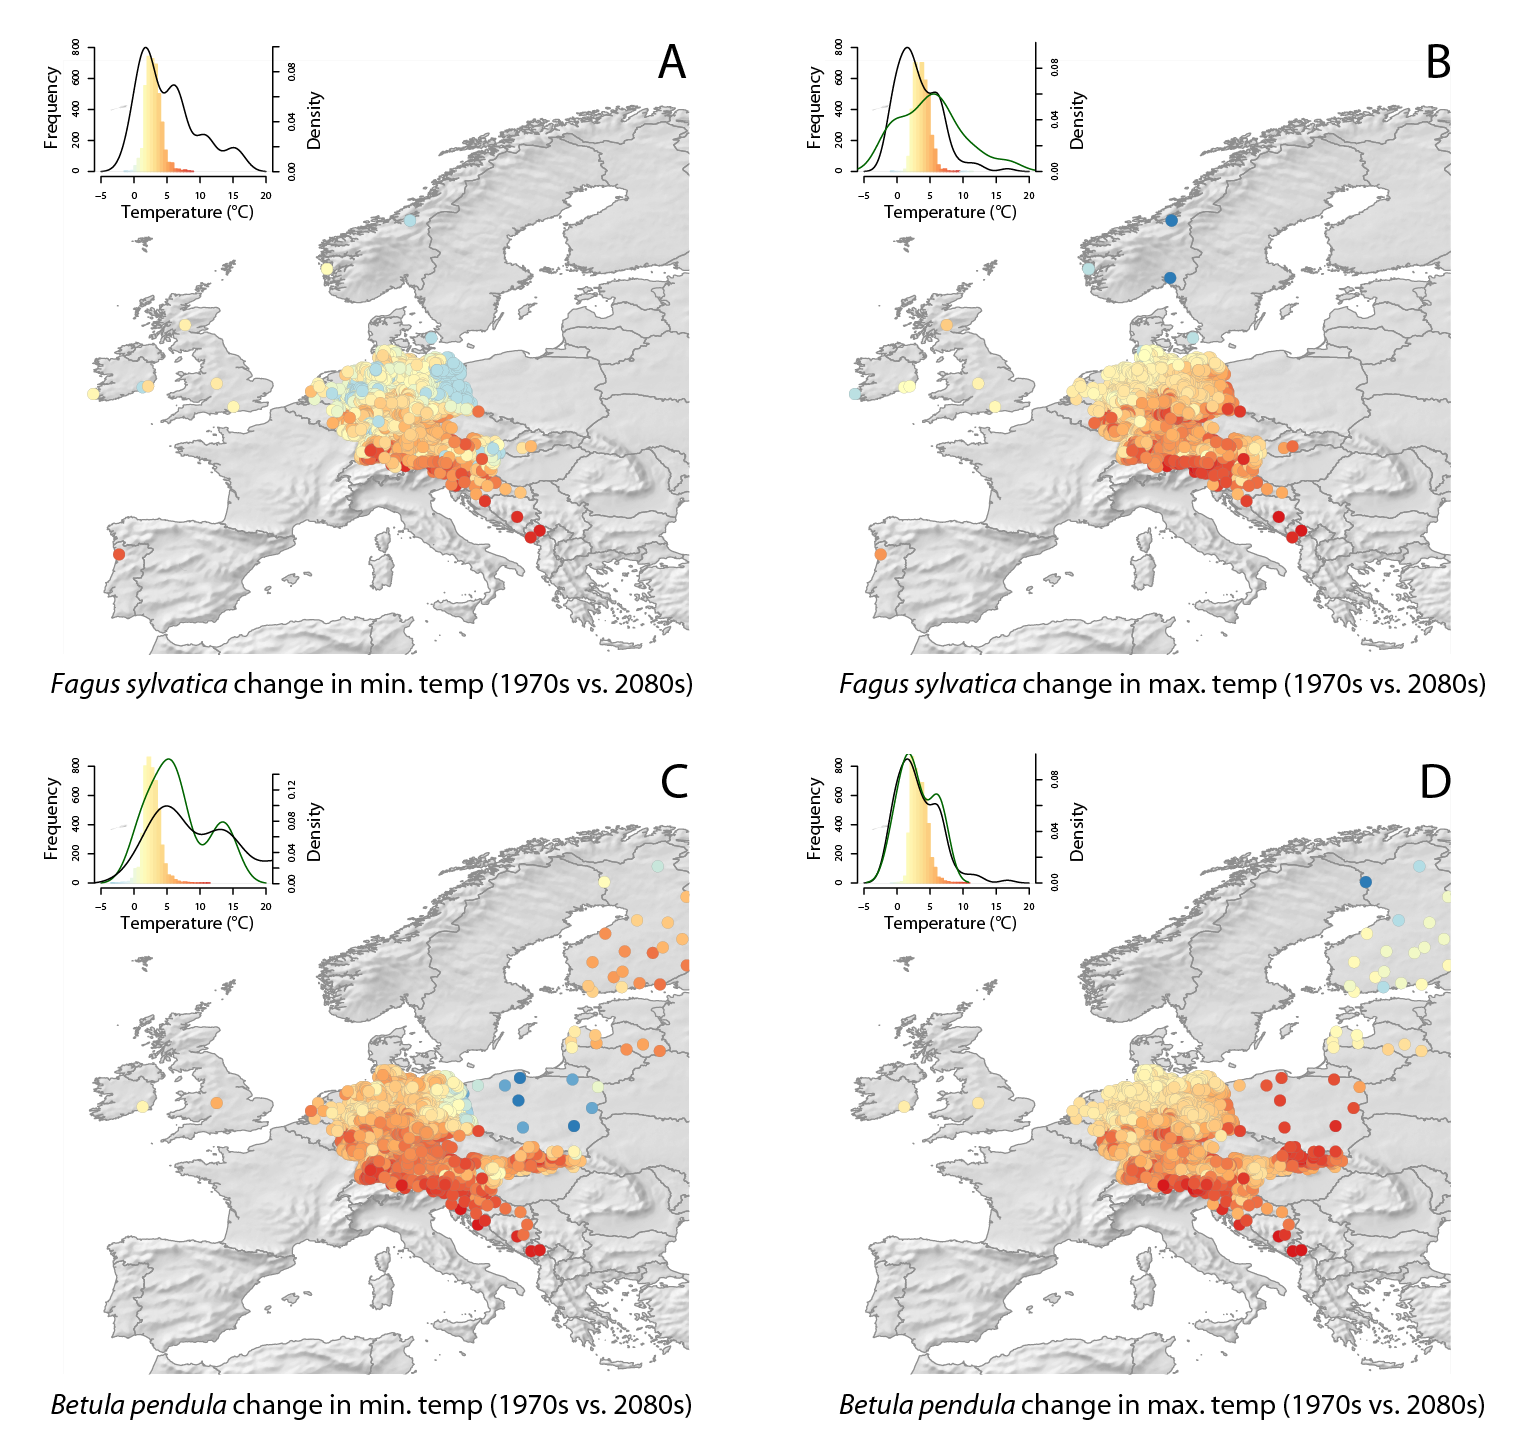
\includegraphics[width=1\textwidth]{figures/Fig1_noblues_densities.png}
\caption{Predicted changes in temperatures relevant to chilling (A, C) and forcing (B, D) compared to a 1970s baseline shown for two species: \emph{Fagus sylvatica} (A-B) and \emph{Betula pendula}. Points represent a PEP725 site with XX data. Inlay plots in the upper left-hand corner of each plot show a histogram of the predicted changes in temperature overlaid with densities of the chilling (A, C) and forcing (B, D) treatments (green lines show the treatments for that exact species, while black lines show across all species; note that for \emph{Fagus sylvatica} there are no chilling treatments of differing temperatures.}
  \label{fig:pep}
\end{figure}
\clearpage


\begin{figure}[t!]
\centering
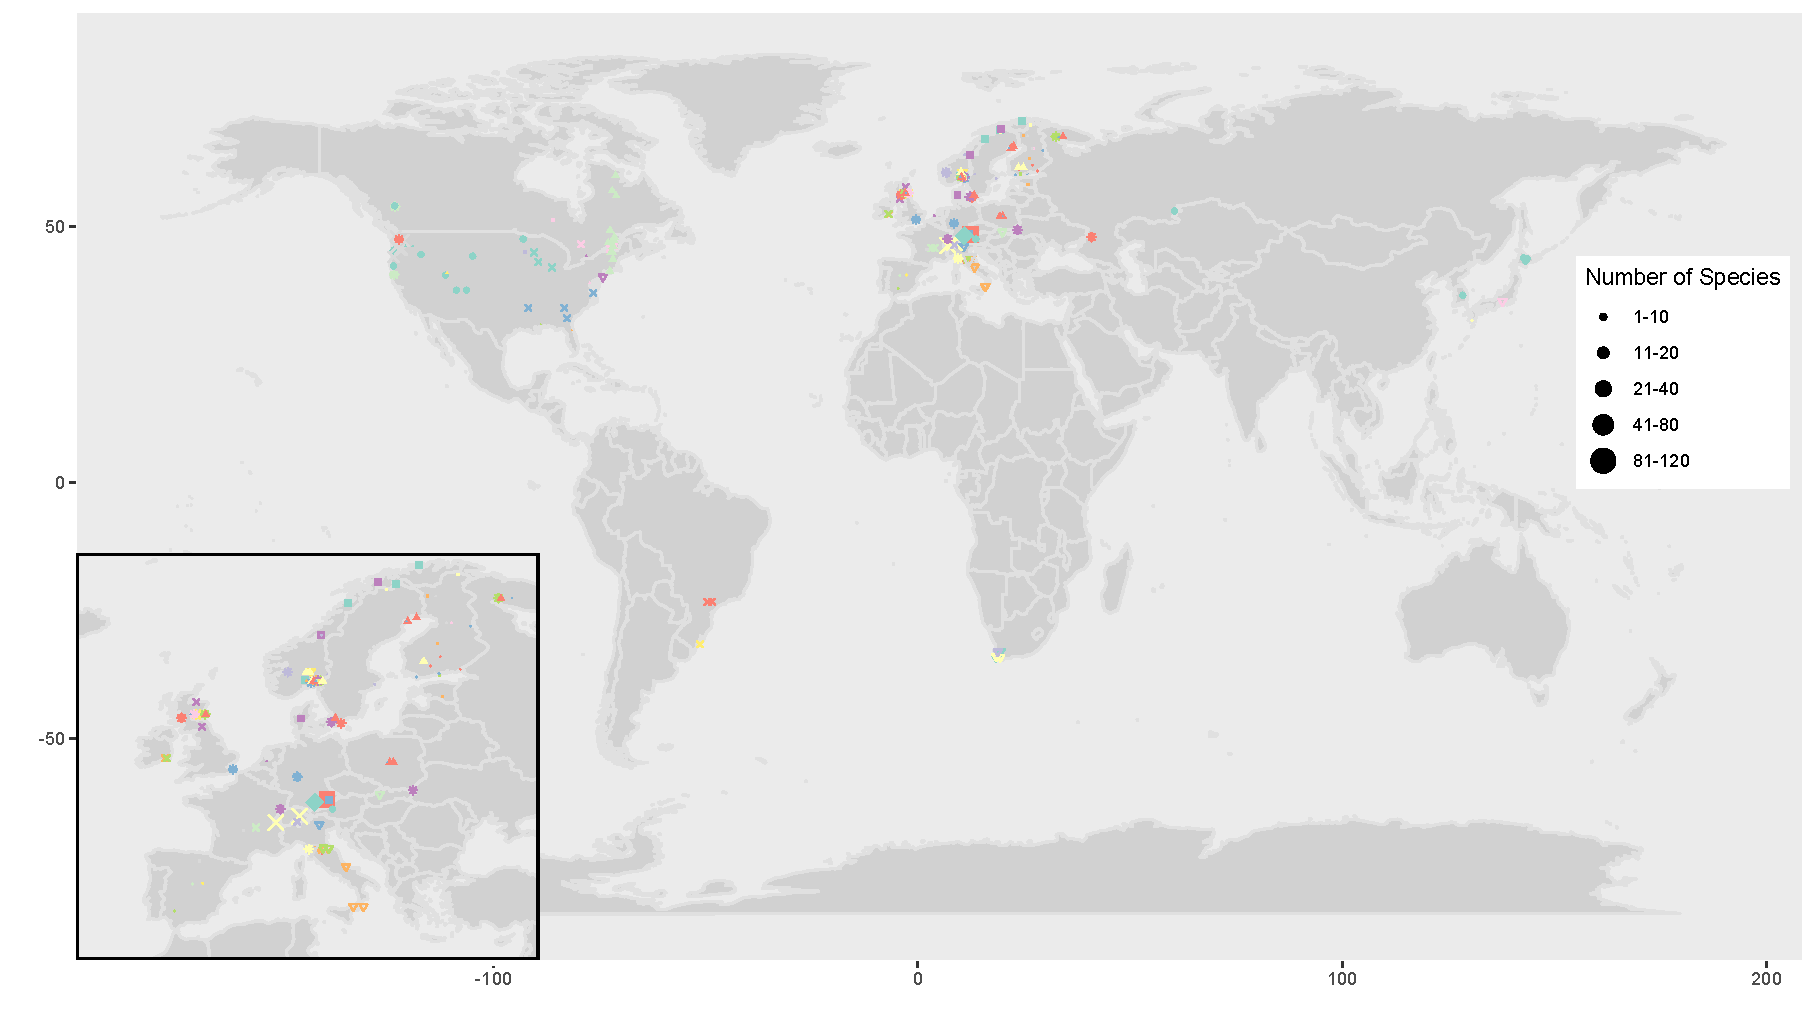
\includegraphics[width=1\textwidth]{..//..//analyses/limitingcues/figures/maps/map_studyspp.pdf}
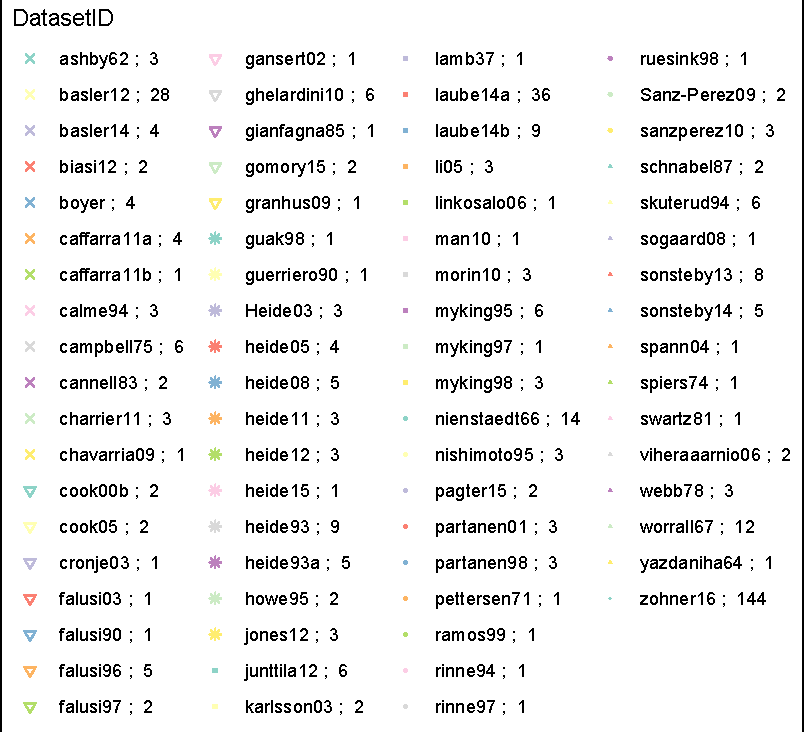
\includegraphics[width=0.5\textwidth]{..//..//analyses/limitingcues/figures/maps/map_studyspp_legend.pdf}

\caption{Overview of the data across space.}
  \label{fig:datamap}
\end{figure}
\clearpage

\begin{figure}[t!]
\centering
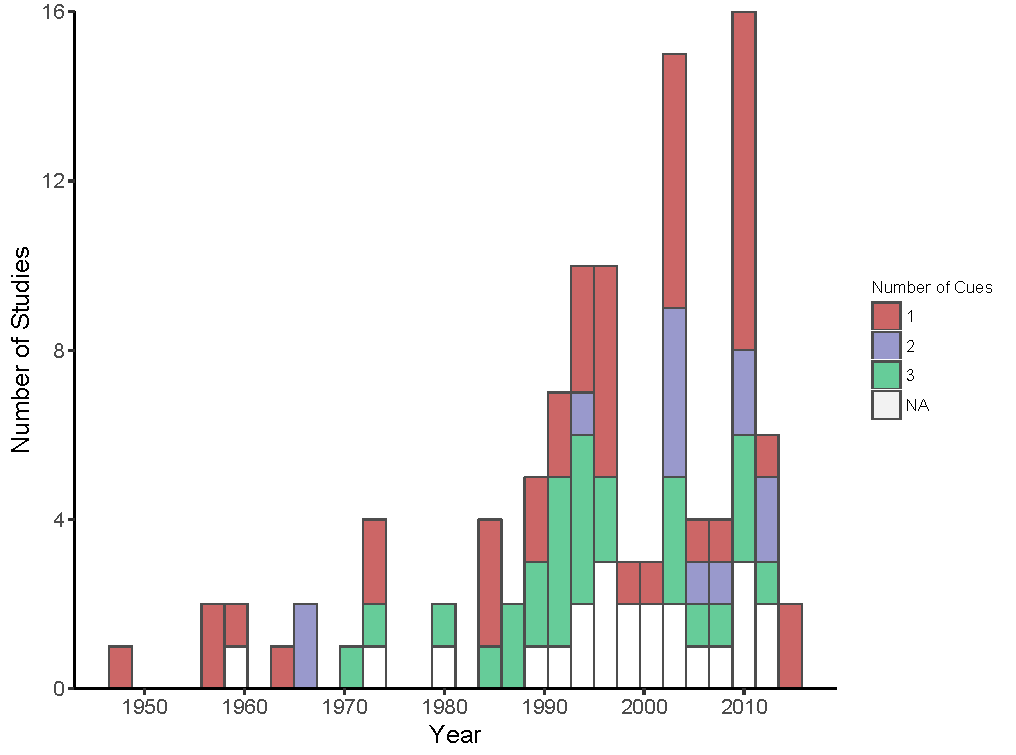
\includegraphics[width=1\textwidth]{..//..//analyses/limitingcues/figures/studyyearcues.pdf}
\caption{Cues manipulated over time.}
  \label{fig:ts}
\end{figure}
\clearpage

\begin{figure}[t!]
\centering
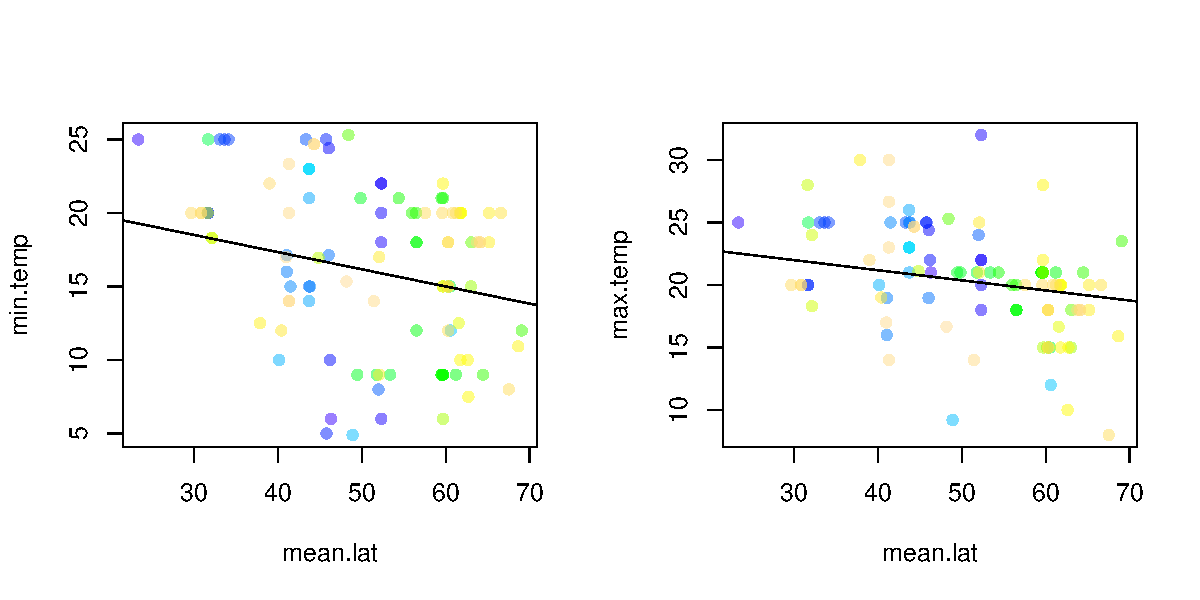
\includegraphics[width=1\textwidth]{..//..//analyses/limitingcues/figures/tempxlatminmaxcorr.pdf}
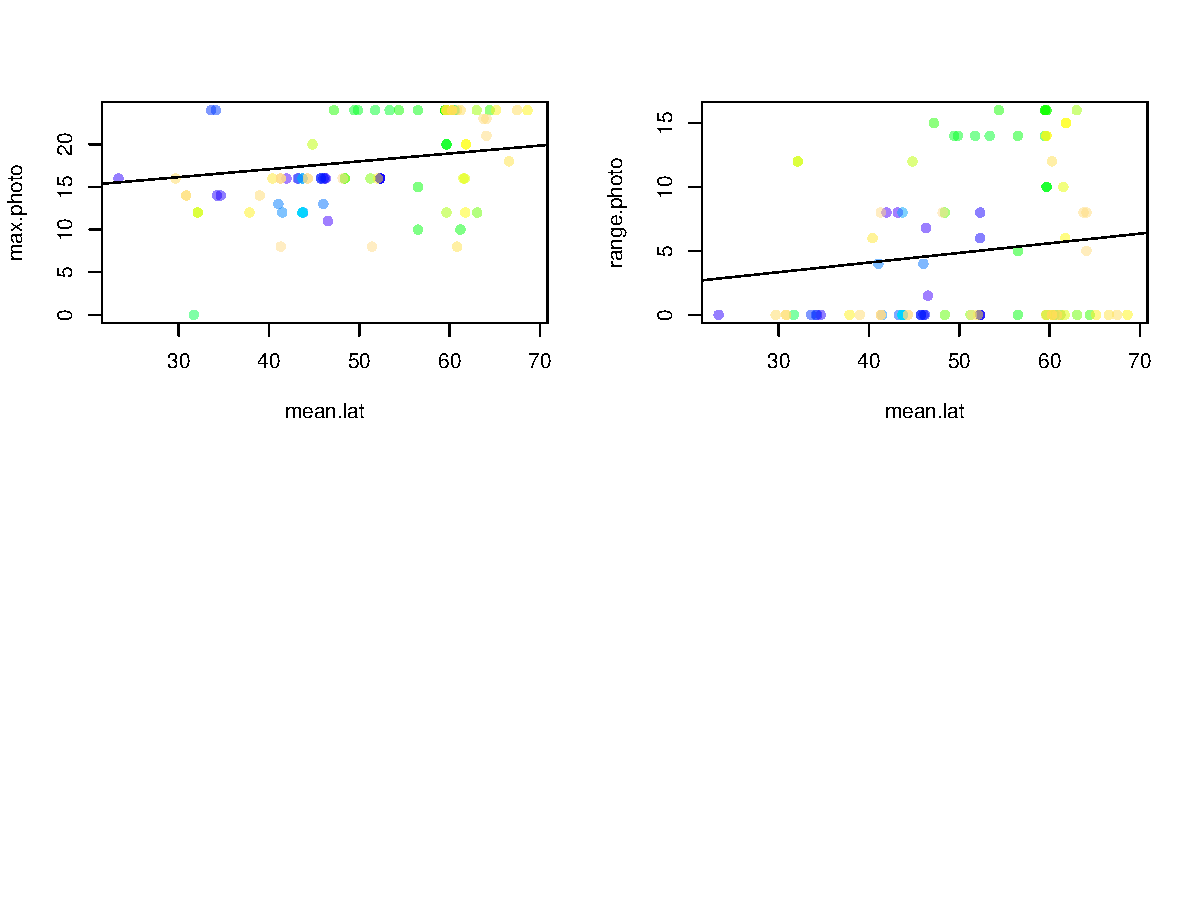
\includegraphics[width=1\textwidth]{..//..//analyses/limitingcues/figures/photoxlatcorr2plots.pdf}
\caption{One correlation with latitude plot? Or more?}
  \label{fig:lat}
\end{figure}
\clearpage

\begin{figure}[t!]
\centering
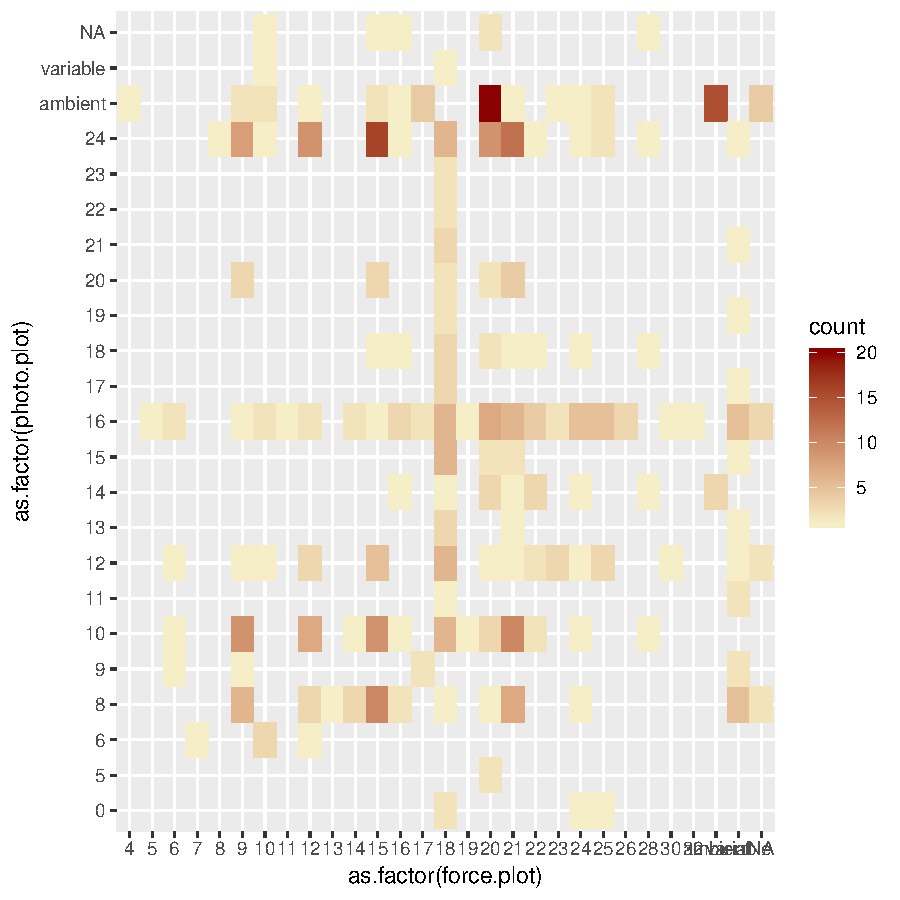
\includegraphics[width=0.3\textwidth]{..//..//analyses/limitingcues/figures/heatmapforcexphoto.pdf}
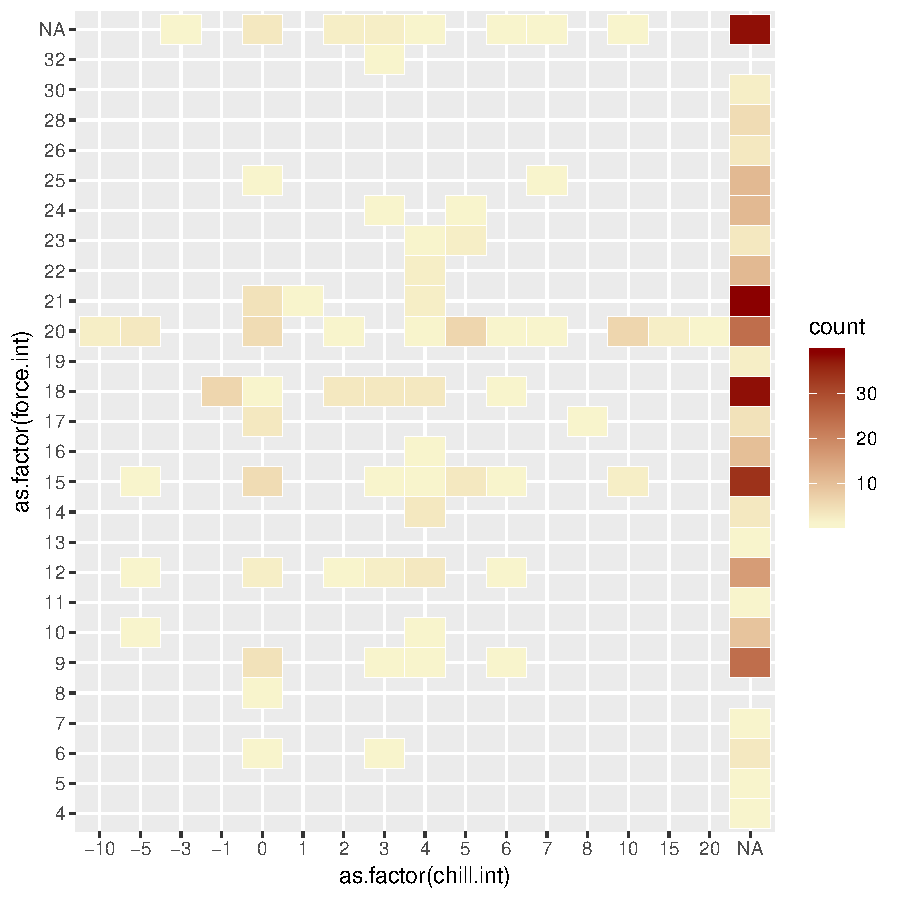
\includegraphics[width=0.3\textwidth]{..//..//analyses/limitingcues/figures/heatmapchillxforce.pdf}
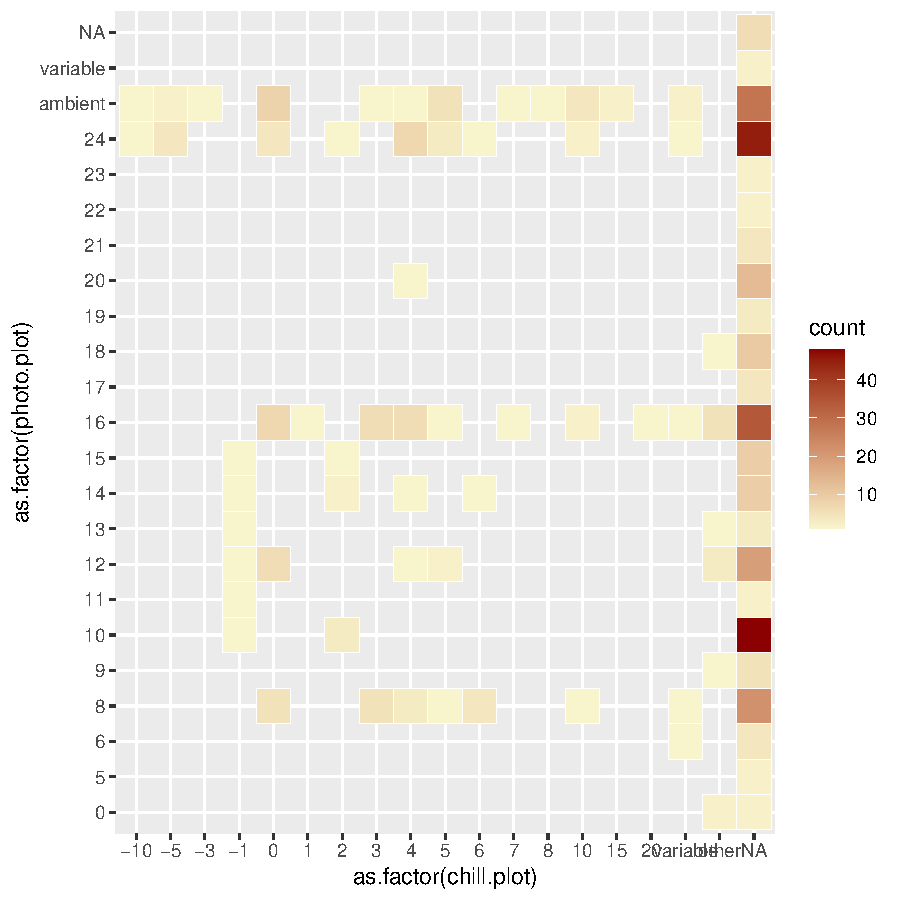
\includegraphics[width=0.3\textwidth]{..//..//analyses/limitingcues/figures/heatmapchillxphoto.pdf}
\caption{Heat maps.}
  \label{fig:heatmaps}
\end{figure}



\end{document}